\chapter{Optimization}
\label{chap:optimization}

One benefit of having a unified algebra for all languages is that a query can be optimized holistically, regardless of which languages it is written in. DortDB comes with a rule-based optimizer; it is also possible to define secondary indices. Even though cost-based optimizers generally perform better, they require statistics about the queried data. DortDB data sources are, by design, schema-less, and no statistics collection takes place. The optimizer thus consists of an extensible set of query rewriting and operator reordering rules.

\section{Secondary indices}
\label{sec:indices}

Unlike single-model databases, multimodel database systems generally require a broader range of index types\cite{mihal2023refining}. As DortDB aims to be extensible and support as many query languages and models as possible, it is necessary to allow the definition of custom index types. Furthermore, different index types might require different conditions to be applied. For example, a hash table index generally requires the query to contain an equality check on a specific attribute, while a range index can also be applied to inequality comparisons. Our solution is to allow the indexing of any expression composed of \texttt{calculation} intermediaries. This means that any \texttt{calculation} that does not contain subqueries is indexable. During the query optimization phase, registered indices receive expressions used to access a data structure and decide whether they are applicable. Currently, the first matching index is selected. This behavior is contained in two replaceable optimizer rules, so developers using DortDB may implement a better algorithm. In figure \ref{fig:tree-indexed-recursion}, an index provided by the Cypher language detects conditions for connected nodes and edges. In figure \ref{fig:tree-index-scan}, a simple hash table index recognizes a relevant equality check.

\begin{figure}[htpb]
    \begin{subfigure}[b]{\textwidth}
    \begin{tcolorbox}[colback=white, colframe=black, boxrule=1pt, arc=0pt]
        \begin{minted}[fontsize=\small]{ts}
// DortDB programmatic configuration:
this.db.createIndex(['t2'], ['a + b / 2'], MapIndex)
        \end{minted}
    \end{tcolorbox}
    \end{subfigure}

    \begin{subfigure}[b]{\textwidth}
    \begin{tcolorbox}[colback=white, colframe=black, boxrule=1pt, arc=0pt]
        \begin{minted}[fontsize=\small]{sql}
SELECT t1.foo, t2.bar FROM t1
JOIN t2
ON t2.a + t2.b / 2 = t1.id
        \end{minted}
    \end{tcolorbox}
    \end{subfigure}

    \medskip

    \begin{subfigure}[c]{248pt}
        \centering
        \frame{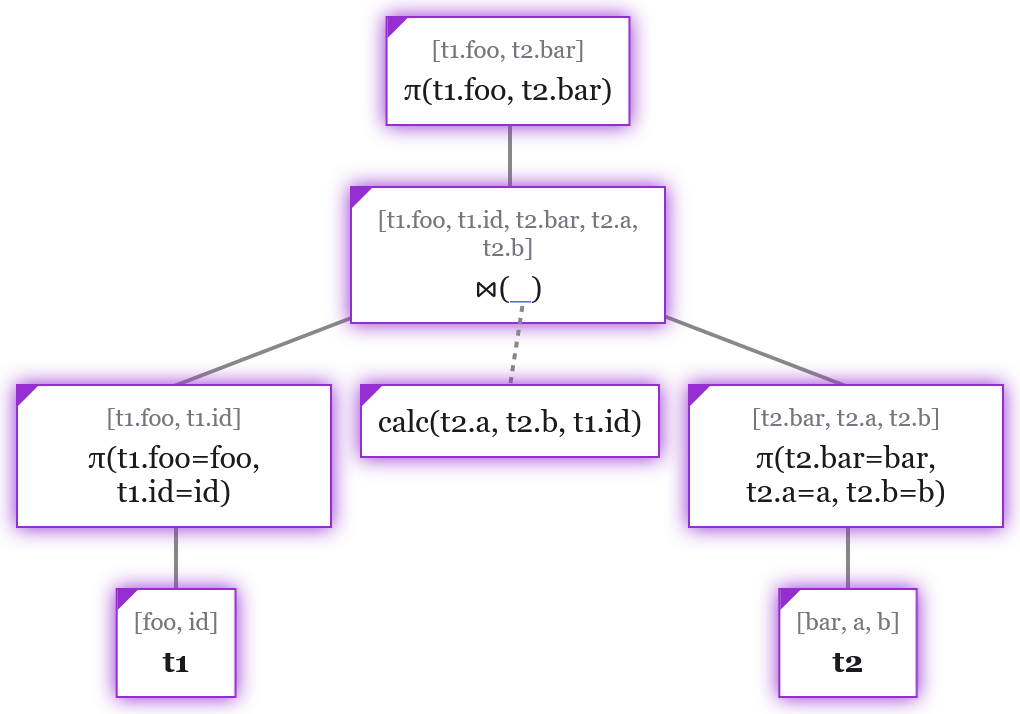
\includegraphics[width=\textwidth]{img/tree-index-scan-before.png}}
    \end{subfigure}\hfill\begin{subfigure}[c]{160pt}
        \centering
        \frame{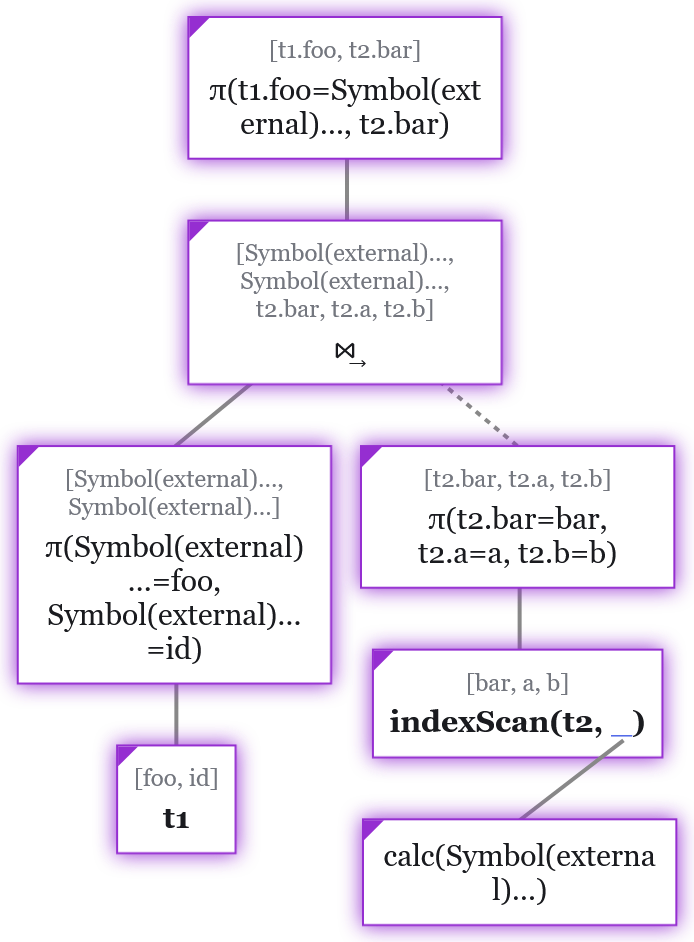
\includegraphics[width=\textwidth]{img/tree-index-scan-after.png}}
    \end{subfigure}
    
    \caption{The registered index recognizes the equality check on the expression it was registered with. Plan before and after the optimization.}
    \label{fig:tree-index-scan}
\end{figure}

\section{Implemented optimizer rules}
\label{sec:optimizer}

The rules in the optimizer follow a simple format. Each rule specifies a set of starting operators. As the rule is processed, the optimizer traverses the query tree from the root down, looking for any operator of a matching type. After such an operator is found, the rule evaluates its \texttt{match} method. If successful, the \texttt{match} function produces bindings, which are supplied to the rule's \texttt{transform} method alongside the subtree starting with the matched operator. The \texttt{transform} method then performs any query rewriting or operator reordering necessary and returns a new subtree, which then replaces the original one.

DortDB comes with a set of implemented rules. During configuration, the user can choose which rules will be used and in what order. In the following sections, the rules will be explained in the order they are applied by default.

\begin{figure}[htpb]
    \begin{subfigure}[b]{\textwidth}
    \begin{tcolorbox}[colback=white, colframe=black, boxrule=1pt, arc=0pt]
        \begin{minted}[fontsize=\small]{sql}
SELECT products.name
FROM products
JOIN (
  LANG cypher
        \end{minted}
        \nestedMintedVspace
        \begin{minted}[style=manni,fontsize=\small]{cypher}
  MATCH (p:person)-[:HAS_INTEREST]->(c:category)
  RETURN p, c.name AS category
        \end{minted}
        \nestedMintedVspace
        \begin{minted}[fontsize=\small]{sql}
) AS interests
ON products.category = interests.category
WHERE interests.p->'id' IN (
  LANG XQuery
        \end{minted}
        \nestedMintedVspace
        \begin{minted}[style=manni,fontsize=\small]{xquery}
  $Invoices/Invoice[
    orderDate < date:sub(now(), interval('1 month'))
  ]/personId/fn:data()
)

        \end{minted}
    \end{tcolorbox}
    \end{subfigure}

    \medskip
    
    \begin{subfigure}{\textwidth}
        \centering
        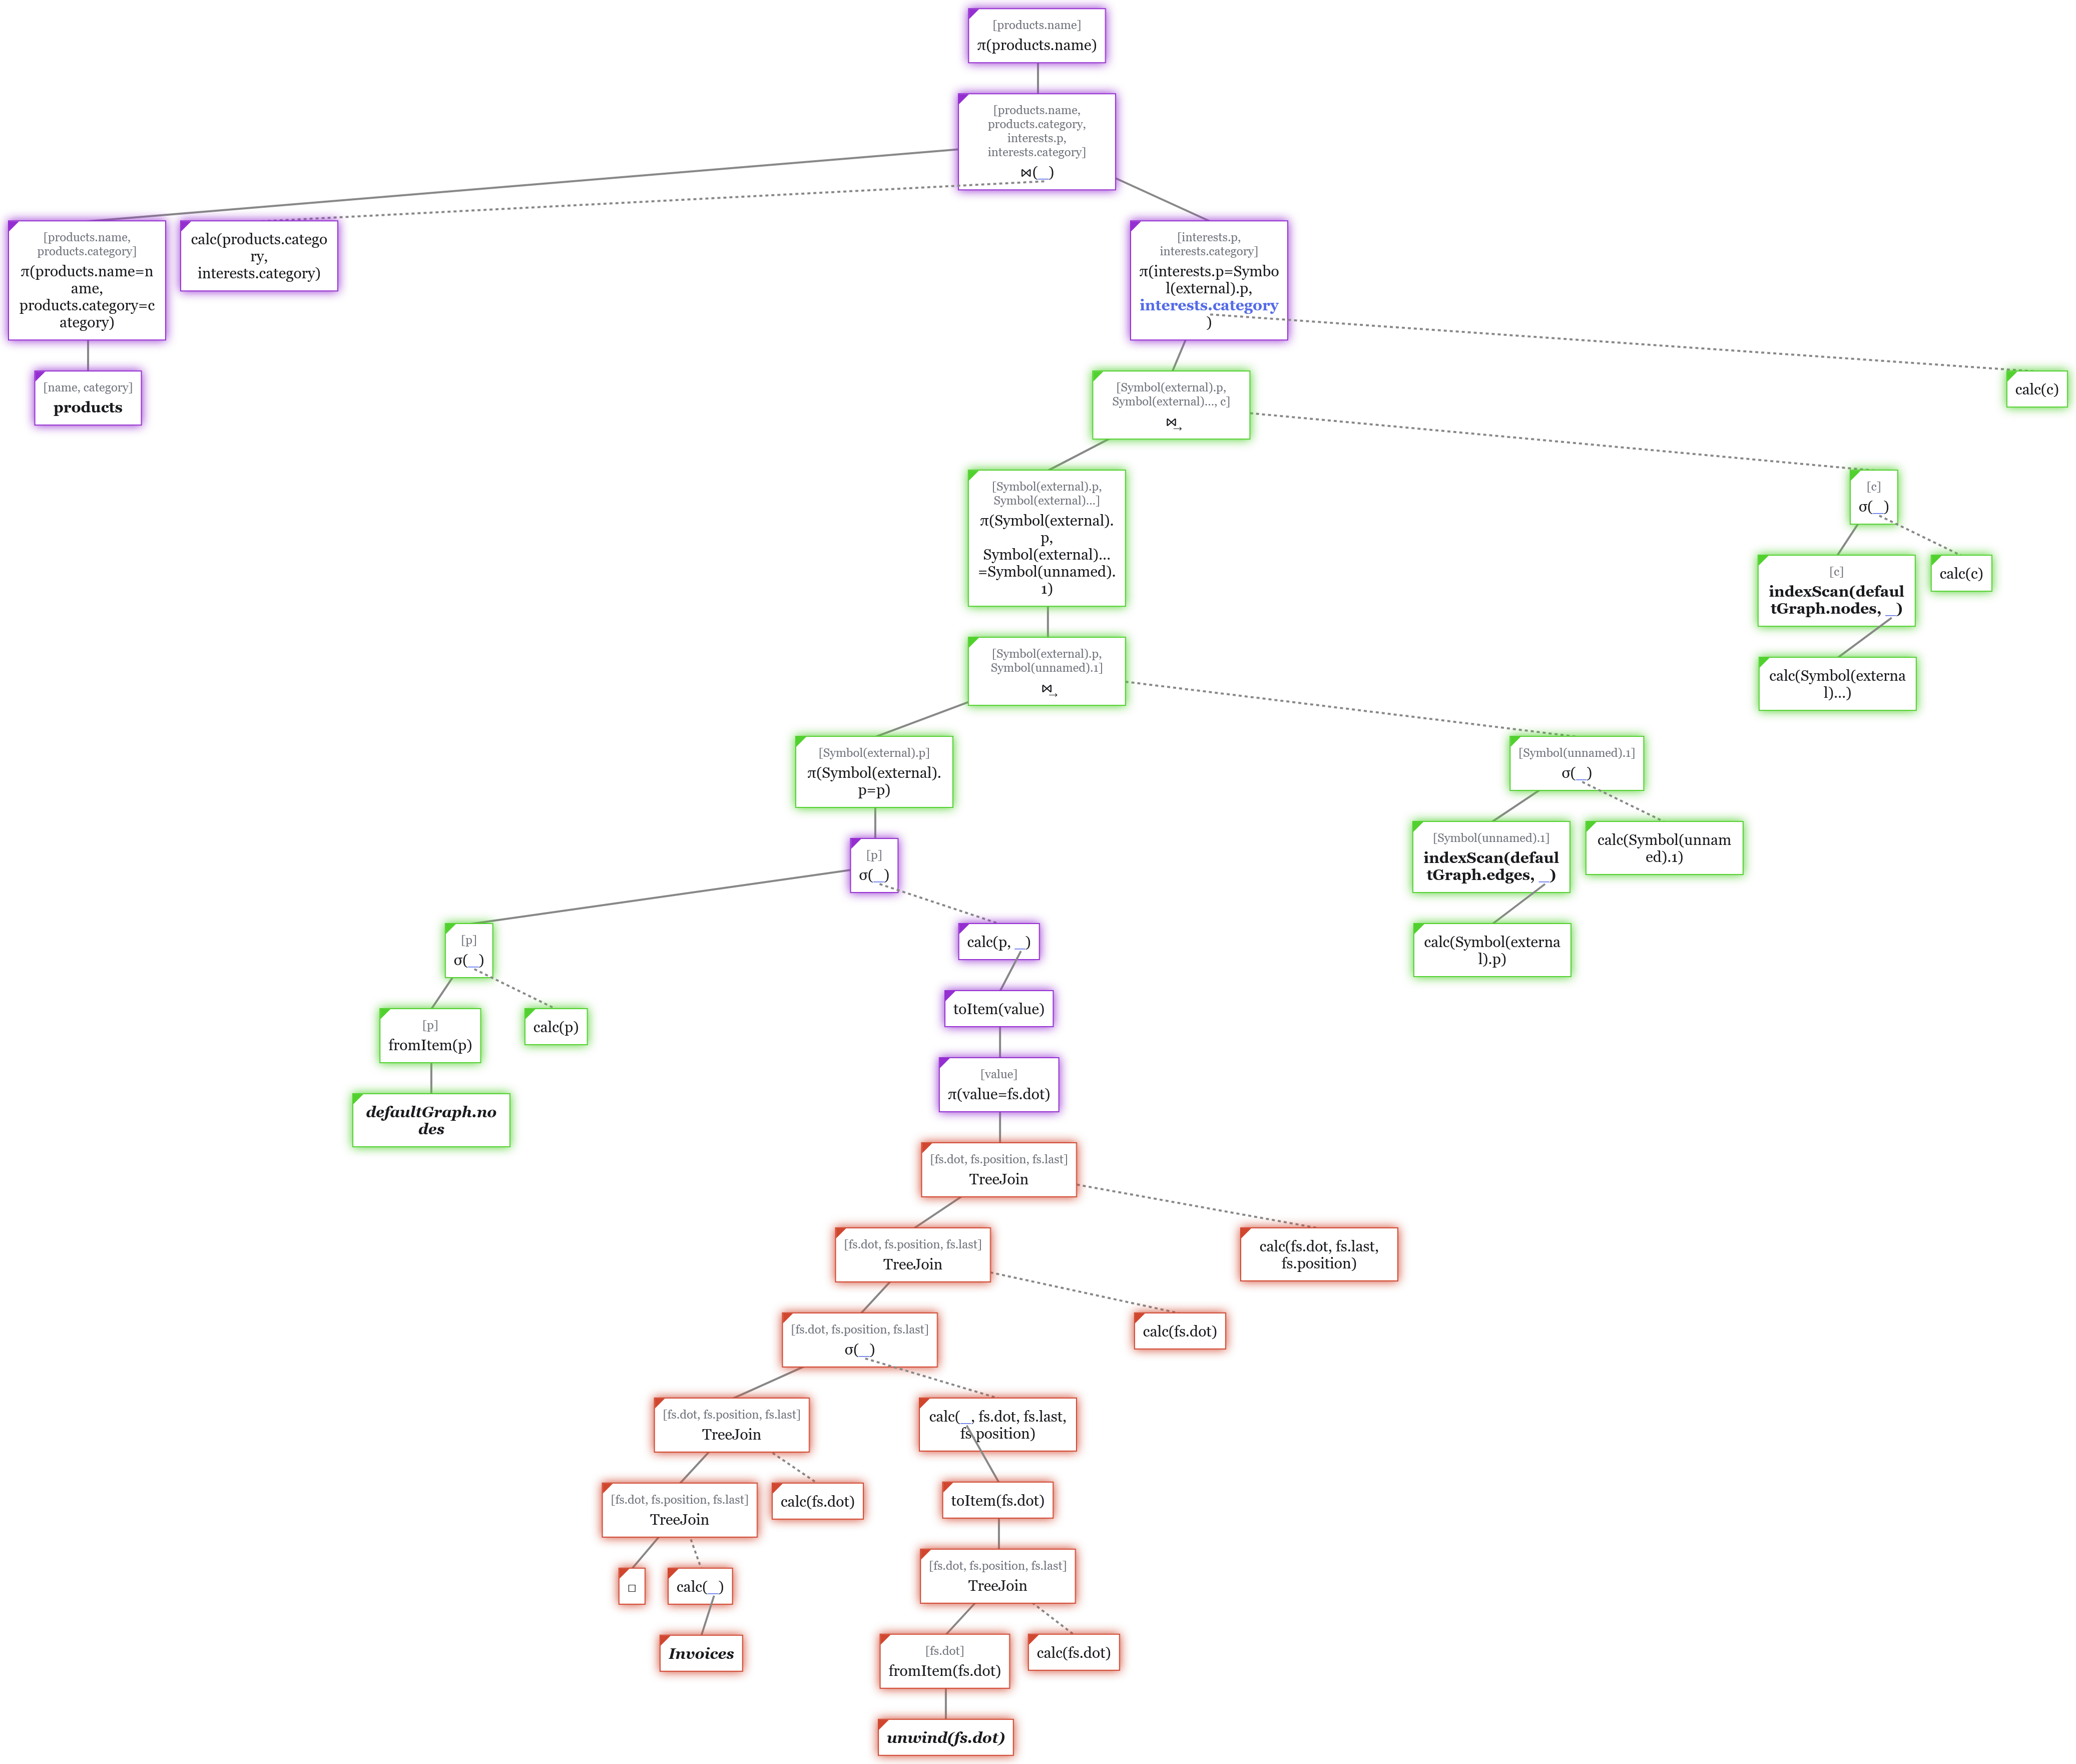
\includegraphics[width=\textwidth]{img/tree-multimodel-optimization.png}
    \end{subfigure}
    
    \caption{Example of how the optimizer works through all the languages at once. Notice the orange-purple subtree, which has been moved into the middle of the green cypher operators. This is the XQuery filter originally specified at the end of the SQL query.}
    \label{fig:tree-multimodel-optimization}
\end{figure}

\subsection{Unnest subqueries}
\label{subsec:unnest-subqueries}

This rule looks for \texttt{calculations} with nested plan operators as arguments. More specifically, it checks for such \texttt{calculations} in \texttt{projections}, \texttt{selections}, \texttt{groupBys} as grouping keys, \texttt{distincts}, and \texttt{orderBys}. The \texttt{calculation} arguments must be set to expect, at most, a single produced value. For example, \mintinline{sql}{(SELECT number FROM table1) + 5} will be matched while \\\mintinline{sql}{val IN (SELECT number FROM table1)} will not.

For each such subquery, the subquery plan operator will be joined as a new attribute using a \texttt{projectionConcat}. The \texttt{calculation} argument will be replaced by the new attribute. The \texttt{projectionConcat} operator will have a flag set for the executor to verify that the operator's \texttt{mapping} really produces at most one value. The \texttt{projectionConcat} will be set as outer unless the \texttt{mapping} is guaranteed to produce a value. An example of such a subquery would be a count-all query.

\begin{figure}[htpb]
    \begin{subfigure}[b]{\textwidth}
    \begin{tcolorbox}[colback=white, colframe=black, boxrule=1pt, arc=0pt]
        \begin{minted}[fontsize=\small]{sql}
SELECT (SELECT number FROM table1) + 5 AS plusfive
FROM table2
        \end{minted}
    \end{tcolorbox}
    \end{subfigure}

    \medskip

    \begin{subfigure}[c]{140pt}
        \centering
        \frame{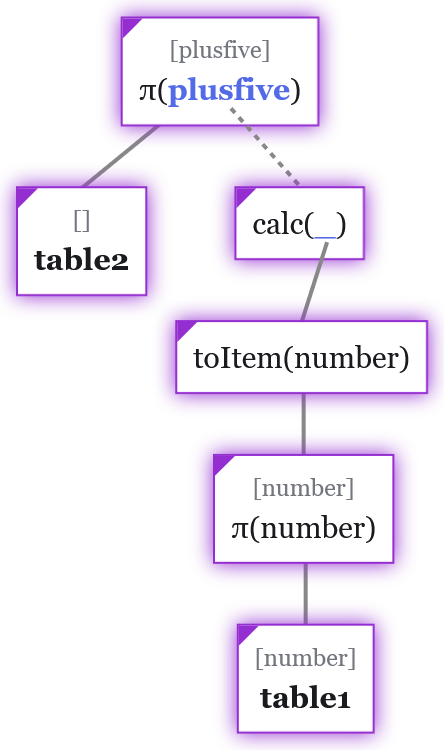
\includegraphics[width=\textwidth]{img/tree-unnest-subqueries-before.png}}
    \end{subfigure}\hfill\begin{subfigure}[c]{268pt}
        \centering
        \frame{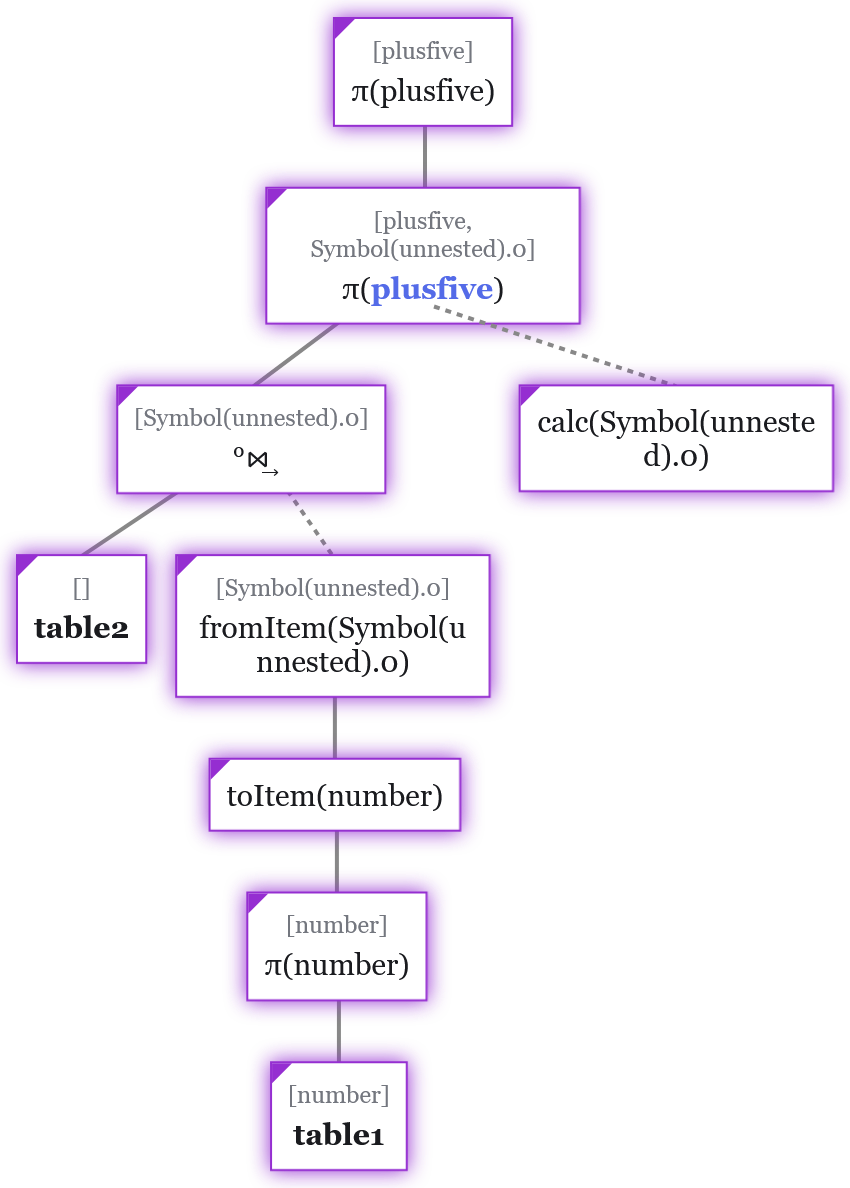
\includegraphics[width=\textwidth]{img/tree-unnest-subqueries-after.png}}
    \end{subfigure}
    
    \caption{An example of an unnested subquery in a \texttt{projection}. The resulting \texttt{projectionConcat} is outer. The redundant \texttt{projection} at the root of the resulting tree is there to ensure the new attribute is stripped away (unnecessary in this case), and will be optimized away by further rules.}
    \label{fig:tree-unnest-subqueries}
\end{figure}

\subsection{Merge to/from items}

As can be seen in figure \ref{fig:tree-unnest-subqueries}, it is possible for \texttt{mapFromItem} to have \texttt{mapToItem} as its source, or vice versa. This happens most often due to query rewriting rules or language switches. The two rules for handling these situations are rather simple -- if \texttt{mapFromItem} is the parent and \texttt{mapToItem} is its source, they become a \texttt{projection} with a single attribute. Otherwise, both operators are simply removed.

\subsection{Pushdown selections}

\texttt{Selections} reduce the cardinality of a tuple stream. It is, therefore, advantageous to process them sooner rather than later. This rule moves \texttt{selections} closer to the leaves of the query tree. The rule considers a continuous sequence of \texttt{selections} and its source operator. The \texttt{selections} which can be pushed below the source are pushed, the rest stay above. The rule is then applied again to the pushed-down \texttt{selections}.

A \texttt{selection} can always be safely pushed below \texttt{orderBy} and \texttt{distinct}. It can also always be pushed down below set operators like \texttt{union} or \texttt{difference}, but it needs to be duplicated and applied to both source branches. \texttt{Selections} can also be swapped with \texttt{projections}, as long as the \texttt{selections} do not rely on any new attributes calculated by the \texttt{projections}. If they depend on renamed attributes, the \texttt{selections} must be modified appropriately. It may not always be possible to rename the \texttt{selection}. When it comes to \texttt{joins} and \texttt{cartesianProducts}, the \texttt{selections} can be pushed into branches that contain all necessary attributes for evaluating the conditions, as long as the \texttt{join} is not left outer and it is not its right branch or vice versa.

\begin{figure}[htpb]
    \begin{subfigure}[b]{\textwidth}
    \begin{tcolorbox}[colback=white, colframe=black, boxrule=1pt, arc=0pt]
        \begin{minted}[fontsize=\small]{sql}
SELECT t1.x, t2.y
FROM t1 JOIN t2
ON t1.id = t2.id AND t1.x > 17
        \end{minted}
    \end{tcolorbox}
    \end{subfigure}

    \medskip

    \begin{subfigure}[c]{214pt}
        \centering
        \frame{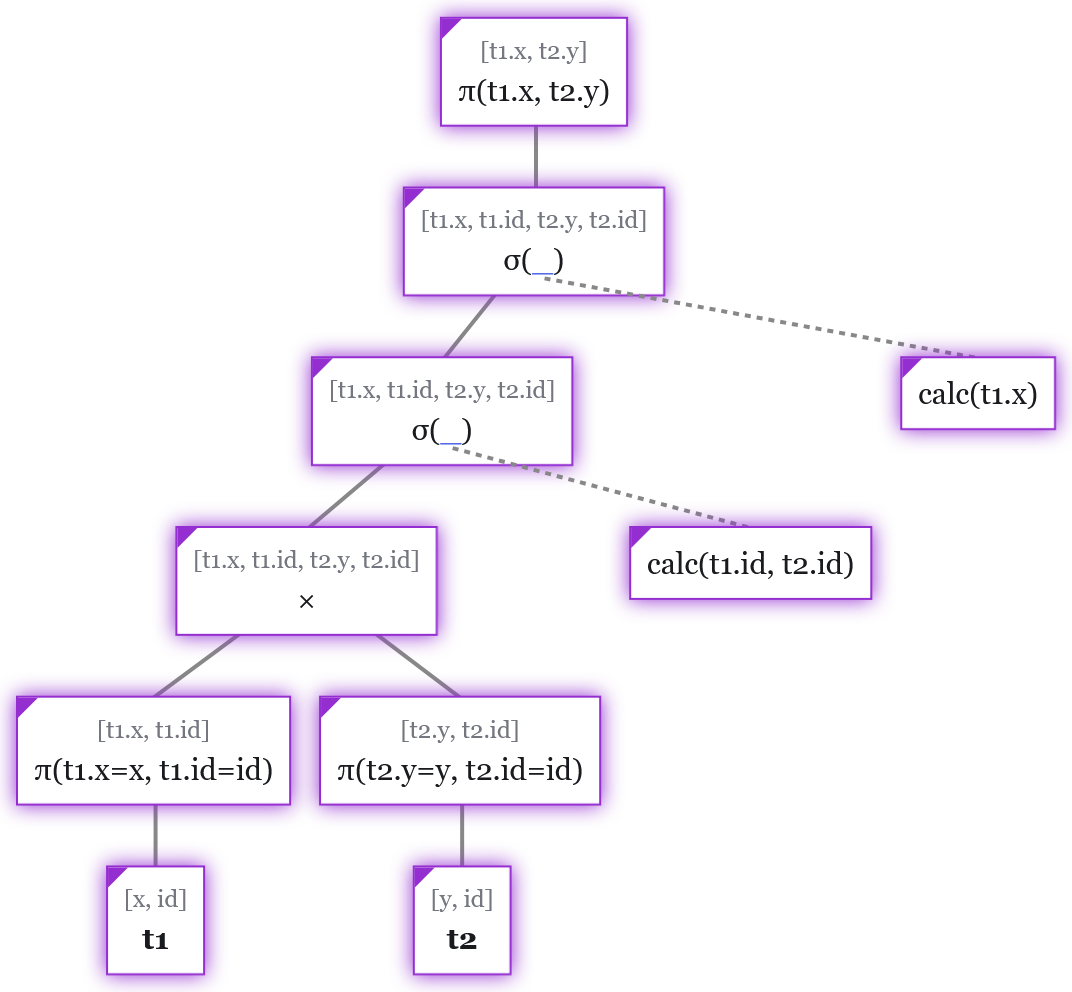
\includegraphics[width=\textwidth]{img/tree-pushdown-selections-before.png}}
    \end{subfigure}\hfill\begin{subfigure}[c]{194pt}
        \centering
        \frame{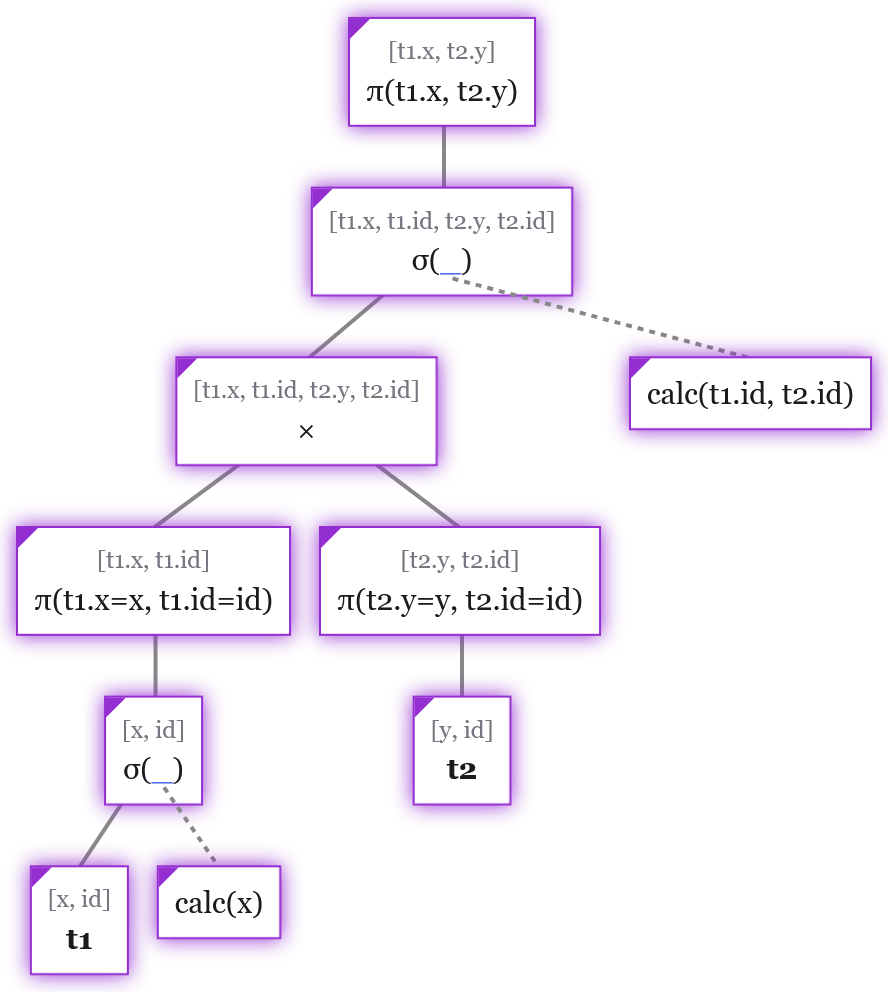
\includegraphics[width=\textwidth]{img/tree-pushdown-selections-after.png}}
    \end{subfigure}
    
    \caption{An example of two \texttt{selections} and a \texttt{cartesianProduct}. The first \texttt{selection} can be pushed into the left branch. The second cannot be pushed anywhere, because it depends on attributes from both branches.}
\end{figure}

\begin{listing}[ht!]
    \begin{minted}[fontsize=\small]{sql}
SELECT t.attr2
FROM (
SELECT t.orig1 AS attr1, t.orig2 AS attr2
FROM t
) AS t
WHERE t.attr1 > (SELECT t.orig1 FROM t2 AS t)
    \end{minted}
    \caption{An overly contrived example where it is not possible to fully push the \texttt{selection} into the \texttt{t2} subquery due to renaming collisions.}
    \label{fig:cannot-rename}
\end{listing}

\subsection{ProjectionConcat to join}

\texttt{ProjectionConcat} may be converted to a \texttt{cartesianProduct} or a left \texttt{join} when its \texttt{mapping} does not depend on the \texttt{source} context (the subquery is not correlated). If the \texttt{projectionConcat} has the \texttt{validateSingleValue} flag set (see section \ref{subsec:unnest-subqueries}), the flag is transferred to the new operator.

\subsection{Products to joins}

This rule merges \texttt{selections} with subsequent \texttt{cartesianProducts} into \texttt{joins}. The resulting \texttt{join} will have multiple conditions instead of a single combined one.

\subsection{Join indices, Index scans}

The two rules responsible for DortDB secondary indices, as described in section \ref{sec:indices}. The first rule detects indexable expressions in \texttt{join} conditions. The \texttt{join} is transformed into a \texttt{projectionConcat} with a \texttt{selection}. The second rule then detects indexable \texttt{selections} and data sources and combines them into \texttt{indexScans}.

\subsection{Merge projections}

This is likely the most complex rule currently implemented in the DortDB optimizer. It combines subsequent \texttt{projections} into a single one when possible. Unused attributes are removed. Calculated attributes are merged as long as the calculation is only referenced once.

\begin{figure}[htpb]
    \begin{subfigure}[b]{\textwidth}
    \begin{tcolorbox}[colback=white, colframe=black, boxrule=1pt, arc=0pt]
        \begin{minted}[fontsize=\small]{sql}
SELECT t.a1, t.a2, t.c1, t.c3 + t.a1 AS c4
FROM (
  SELECT t.a1, t.a2, t.c1, t.c2 * 2 AS c3, t.unused
  FROM (
    SELECT a1, a2, a3 * 2 AS c1, a4 * 2 AS c2, unused
    FROM t
  ) AS t
) AS t
        \end{minted}
    \end{tcolorbox}
    \end{subfigure}

    \medskip

    \begin{subfigure}[c]{234pt}
        \centering
        \frame{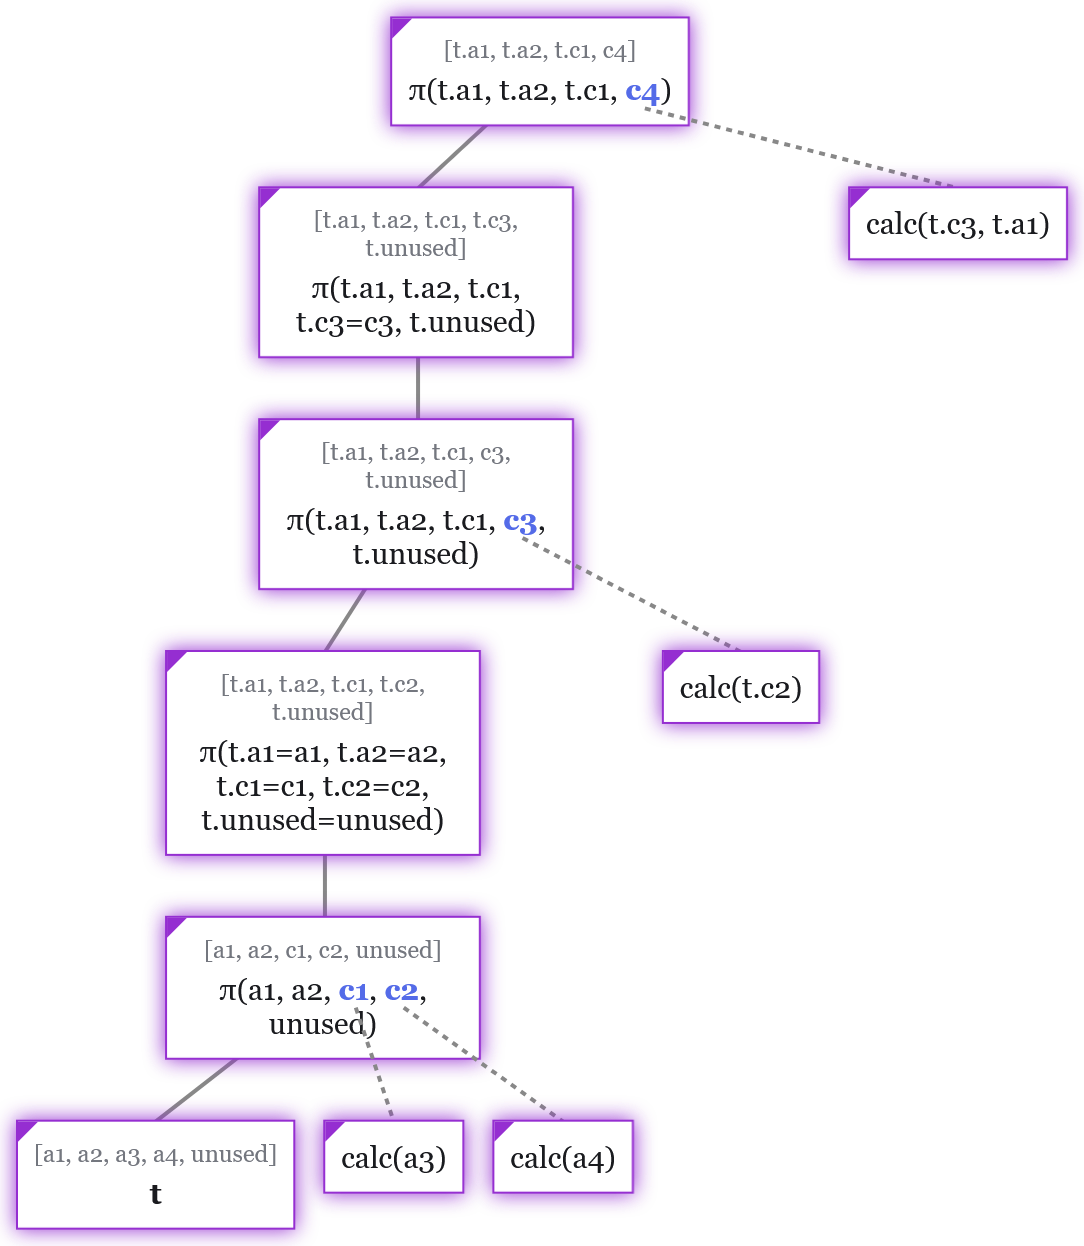
\includegraphics[width=\textwidth]{img/tree-merge-projections-before.png}}
    \end{subfigure}\hfill\begin{subfigure}[c]{174pt}
        \centering
        \frame{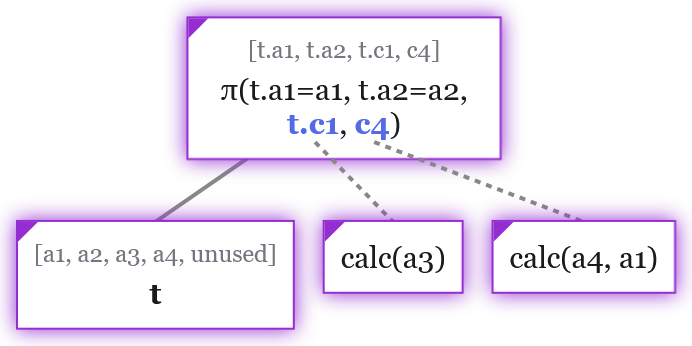
\includegraphics[width=\textwidth]{img/tree-merge-projection-after.png}}
    \end{subfigure}
    
    \caption{An example of multiple merged \texttt{projections}. The \texttt{unused} attribute is removed. Calculated attributes are merged into more complex calculations. If the outer query selected \texttt{t.c1} twice, some merging would be prevented in order to avoid recomputing potentially expensive calculations multiple times. The final query tree would contain two \texttt{projections}.}
\end{figure}

\section{Calculation building}
\label{sec:calc-building}

\texttt{Calculations} are usually created from intermediary plan operators such as \texttt{FnCalls}. This process aims to create a single final callable. \texttt{FnCalls} can be marked as \textit{pure}. If arguments of pure \texttt{FnCalls} are constant (represented by \texttt{literal} plan operators), the function is precomputed and replaced by a \texttt{literal} containing the result. This way, redundant computation may be avoided. During the building process, SQL-style \texttt{quantifiers} combined with specific comparison operators are optimized using rules specified in \cite{holsch2016optimization}.